\input{wg21common}

% Footnotes at bottom of page:
 \usepackage[bottom]{footmisc} 

% Table going across a page: 
 \usepackage{longtable}

 % Start sections at 0
% \setcounter{section}{-1}

\begin{document}
\title{Contracts for C++: Revisiting contract check elision and duplication}
\author{ Timur Doumler \small(\href{mailto:papers@timur.audio}{papers@timur.audio}) 
}
\date{}
\maketitle

\begin{tabular}{ll}
Document \#: & D3228R0 \\
Date: &2024-04-10 \\
Project: & Programming Language C++ \\
Audience: & SG21
\end{tabular}

\begin{abstract}
This paper attempts to add some structure to the discussion whether the Contracts MVP should retain the rule that checked contract assertions are allowed to be evaluated any number of times when checking a contract predicate, or tighten it to require exactly one evaluation, or possibly some interval of allowed values. We list the different conflicting design requirements and the possible specification solutions, and provide an analysis of which solutions satisfy which design requirements.
\end{abstract}

%%%%%%%%%%%%%%%%%%%%%%%%%%%%%%%%%%%%%%%%%%%%%

\section{Introduction}
\label{sec:intro}

The current Contracts MVP \cite{P2900R6}, as forwarded by SG21 to EWG and LEWG for design review, specifies that for a \emph{checked} contract assertion, the predicate evaluation may be elided if the compiler can prove that the result of such an evaluation would be \tcode{true} or \tcode{false}. Further, it specifies that at any point within a contract assertion sequence, any previously evaluated contract assertions may be evaluated again. Effectively this means that, if a predicate has observable side effects, those side effects may occur zero, one or more times, with no upper bound on the number of possible evaluations.

The design review of \cite{P2900R6} at the March 2024 WG21 meeting in Tokyo revealed several issues with this approach:
\begin{itemize}
\item A contract assertion that will exhibit undefined behaviour after a number of repeated assertions (say, repeated signed integer addition) can be considered to exhibit undefined behaviour always, as there is no specified upper bound on the number of evaluations;
\item Low-latency and real-time systems require a deterministic upper bound on the runtime complexity of a contract assertion;
\item For some safety-critical systems, a deterministic upper bound is not sufficient; instead, a guarantee is required that a checked assertion is evaluated a known, deterministic number of times.
\end{itemize} 

\cite{P3119R0} attempts to address the first two issues by proposing that the number of times a contract assertion may be repeated in a contract assertion sequence is an implementation limit, i.e. introducing an implementation-defined upper bound, and recommends a value of 64. However, \cite{P3119R0} does not address the third issue.

\pagebreak % MANUAL %%%%%%%%

 A poll taken by EWG in Tokyo revealed that a significant number of people prefer that contract assertions should \emph{not} be allowed to be evaluated more than once (results see \cite{D3197R0}, Poll 7). This poll suggests that the solution proposed in \cite{P3119R0} is insufficient and we may have to address the third issue as well if we want to get the Contracts MVP into C++26. \cite{D3197R0} proposes that this issue be rediscussed in SG21. This paper serves to inform that discussion.

%%%%%%%%%%%%%%%%%%%%%%%%%%%%%%%%%%%%%%%%%%%%%

\section{Scope of this paper}

This paper does not propose any concrete change to the Contracts MVP. Instead, it lists the different conflicting design requirements and the possible specification solutions, and provides an analysis of which solutions satisfy which design requirements. The intent of the paper is to add some structure to the discussion and to highlight the engineering tradeoffs that each solution involves, to help SG21 reach consensus.

We do not consider \emph{unchecked} contract assertions (those having the \emph{ignore} evaluation semantic), as such evaluations do not involve evaluating the predicate.

Further, we do not consider contract predicates that have no observable side effects. Under the as-if rule, it is unobservable whether such ``pure'' predicates are evaluated zero, one, or multiple times, as long as the compiler has correctly determined whether the result of such an evaluation would be \tcode{true} or \tcode{false}. We therefore only consider contract predicates that have \emph{observable side effects} when evaluated.

Finally, we do not consider contract assertions whose evaluation may end up being elided because of undefined behaviour occurring either during evaluation of the predicate itself or elsewhere in the program. We only consider programs that would have well-defined behaviour when the predicate is evaluated once.


%%%%%%%%%%%%%%%%%%%%%%%%%%%%%%%%%%%%%%%%%%%%%

\section{Prior work}

This topic has already been extensively discussed in SG21. The concerns regarding low-latency and real-time systems and the results of the EWG poll constitute new information, which is why the topic needs to be re-discussed again, however it is useful to be aware of the long history of this discussion.

In C++2a Contracts \cite{P0542R5}, as adopted into the C++20 Working Draft, the issue of contract check elision and duplication did not arise, because evaluating a contract predicate that has observable side effects was specified to be undefined behaviour.

The paper \cite{P1670R0} proposed to change C++2a Contracts to make predicates with side effects well-defined but allow elision of the predicate evaluation. This paper was never adopted into the C++20 Working Draft because Contracts were removed from it before the paper was considered, however it made its way into an early version of the Contracts MVP \cite{P2388R4}, which additionally allowed to \emph{duplicate} the evaluation. This went through several iterations. \cite{P2388R0} allowed to elide or duplicate all (as opposed to ``some') side effects of the evaluated predicate, as long as this does not affect the result of that evaluation. \cite{P2388R3} relaxed this to allow eliding or duplicating such side effects per subexpression of a predicate. \cite{P2521R5} strengthened it again to ``all side effects''.

Later, \cite{P2751R1} proposed a more loose model. Instead of allowing elision or duplication, it deliberately made \emph{unspecified} the number of evaluations of the predicate of a checked contract; i.e. each such predicate may be elided, evaluated once, twice, or even more times, with no specified upper bound. This model was adopted for the MVP by SG21 consensus. A counter-proposal, \cite{P2756R0}, which proposed that the predicate of a checked contract should be evaluated exactly once, failed to get consensus. Another proposal, \cite{P2680R1}, which proposed a design direction whereby contract predicates with side effects would be ill-formed by default, failed to get consensus as well. \cite{P2751R1} lists the poll results. \cite{P2570R2} provides a large amount of additional discussion regarding predicates with side effects.

%%%%%%%%%%%%%%%%%%%%%%%%%%%%%%%%%%%%%%%%%%%%%

\section{Design requirements}
\label{sec:reqs}

In this section, we summarise the different, partially conflicting design requirements that have motivated different proposals in this space.

\subsection{Deterministic number of evaluations}
\label{subsec:determ}

There are several reasons to guarantee a deterministic number of times that the predicate is evaluated, i.e. to disallow both elisions and duplications. Such deterministic behaviour is a requirement in some safety-critical systems, which may be unable to use Contracts at all unless this requirement is satisfied.

In addition, a deterministic number of evaluations is required if we wish to minimise the amount of implementation-defined and unspecified behaviour added to the C++ language by the Contracts MVP, which is something that has been brought up as a concern in EWG.

Finally, \cite{P2756R0} argues that a deterministic number of evaluations, and specifically the choice of exactly one evaluation, has some other desirable properties: it is simple, intuitive, has existing practice (\tcode{assert} and similar macros), and is easy to reason about. For example, a user might want to rely on the number of evaluations for a counter counting how many times the assertion has been checked. 

Such uses of assertions can be found in practice. For example, one might want to add an assertion counting the number of times a function is calling itself recursively, and report a contract violation if this recursion depth exceeds a fixed limit. At the same time, incrementing the counter when assertions are ignored might be undesirable for performance reasons, which means that the counter needs to be incremented inside the predicate. Such an assertion will only work correctly if the user can rely on the predicate being evaluated exactly once when the predicate is checked. It is reasonable to assume that many users will expect this behaviour when writing such an assertion, as this is the behaviour they are used to from \tcode{assert} and similar macros. Specifying anything else than exactly one evaluation means that when such an assertion is upgraded from \tcode{assert} to \tcode{contract_assert}, the program can silently break: if evaluations are elided or duplicated, the assertion can end up failing when it should pass, or passing when it should fail, potentially leading to undefined behaviour, and the user does not even get a compiler warning. In practice, such cases will probably be rare, as most of the time such a counter variable used in a predicate will be maintained in an \tcode{\#ifndef NDEBUG} block to avoid paying for the variable in unchecked builds, which means that an attempt to upgrade the assertion to \tcode{contract_assert} will result in a compile error.

\subsection{Deterministic upper bound on number of evaluations}
\label{subsec:upper}

Some low-latency systems have less strict requirements and do not require full deterministic behaviour, but do require a deterministic upper bound on the runtime complexity of a contract assertion. These systems may be unable to use Contracts at all unless this requirement is satisfied.

In addition, without such a deterministic upper bound, a contract assertion that will exhibit undefined behaviour after a number of repeated assertions (say, repeated, accumulating signed integer addition) can be considered to exhibit undefined behaviour always; a particularly hostile compiler may treat such contract assertions as unreachable code while being conforming. Both of these issues are discussed in more detail in \cite{P3119R0}.

There are two ways to specify such an upper bound: either specify a concrete number in the Standard (for example, ``at most two evaluations''), or merely specify that an implementation has to define \emph{some} deterministic upper bound but leave the actual number unspecified. The latter is proposed by \cite{P3119R0}. To what degree either option is acceptable instead of the stricter ``deterministic number of evaluations'' guarantee will depend on the concrete use case.

\subsection{Allow duplications}
\label{subsec:ville}

\cite{P2751R1} lists several reasons to allow duplication of predicate evaluations, but the main use case is to allow the implementation to perform both caller- and callee-side checking while preserving ABI compatibility. Note that only a subset of contract checks can be implemented caller-side\footnote{Note that, if we adopt the proposed design in \cite{P3097R0} and \cite{P3165R0} for supporting function contract assertions on virtual functions, the reverse will also become true: only a subset of contract checks can be implemented callee-side. In particular, checks for function contract assertions of the statically called function in a virtual function call can only be generated caller-side as the statically called function is unknown to the callee.}. Some contract checks must be performed callee-side, for example, when a function is called indirectly, such as through a function pointer or a facility like \tcode{std::function}\footnote{In such scenarios, a callee-side check can be generated only if the compiler front-end sees the function contract assertion related to the function call, i.e. it knows which function will be called and can see the declaration of that function.}, when inside a contract predicate a function is called that is located in another module and is not exported by that module, or when checking postconditions in the Microsoft ABI, as this ABI performs argument destruction callee-side and postcondition checks are guaranteed to happen before argument destruction. 

Now, consider a shared library that has function contract assertions on its function declarations, and an application that uses this library by compiling against a static library header and then dynamically loading a compiled library binary. The developer of the application needs to have the choice of compiling the application with caller-checks either disabled or enabled (the latter resulting in the caller-checkable subset of the library checks being checked, which can be useful to diagnose problems). Likewise, the provider of the shared library needs the choice to ship the compiled library binary with callee-side checks disabled or enabled (the latter being a ``hardened'' version of the library). Either version of the application should be able to use either version of the library binary without having to recompile and re-link. The combination of the application having caller-side checks enabled and the library having callee-side checks enabled will result in some library checks being checked twice.

We can consider implementation strategies that would allow this use case while also guaranteeing that contract checks be evaluated exactly once (or not more than once), but such strategies come with tradeoffs. One possible strategy would be to compile the library binary such that each function with precondition or postcondition assertions has two entry points, one that performs the callee-side check and one that does not. However, this can significantly increase the amount of symbols in the binary, and requires a change to the ABI. Another possibility is to compile the library such that the choice whether to perform callee-side checks is made dynamically, but this incurs additional runtime overhead and again requires a change to the ABI.

For some users, the tradeoffs of either strategy will be unacceptable: a global ABI break might make this approach undeployable, and in a world where some C++ applications require tens of gigabytes of memory to link due to the sheer amount of symbols, there is a strong incentive to avoid adding more symbols. Further, there is currently no implementation experience for either strategy\footnote{Caller-side checking itself does not have implementation experience either, but it is arguably somewhat less theoretical, because compilers know how to parse the function contract specifiers of a function declaration and rewrite a function call \tcode{f()} into a caller-side checked function call such as \mbox{\tcode{(pre_check() ? f() : abort())}}.}. Avoiding such tradeoffs however requires us to either explicitly allow duplication of predicate evaluations, or to place this use case outside of the scope of the C++ Standard and treat support for it as a non-conforming vendor extension, as we do for example for \tcode{-fno-exceptions}.

\subsection{Allow elisions}
\label{subsec:elisions}

One might want to allow eliding contract predicates along with their observable side effects, in a fashion similar to copy elision, if the compiler can prove that the result of the elided evaluation would be \tcode{true} or \tcode{false}. For example, if a function \tcode{f} has a checked precondition assertion \tcode{pre(x)}, and immediately after that, as the first statement in the body of \tcode{f}, another function \tcode{g} with a functionally equivalent precondition assertion is called, eliding the latter assertion would avoid unnecessarily evaluating the expression \tcode{x} twice. This is discussed in more detail in \cite{P2751R1}.

\subsection{Allow more than two repetitions}
\label{subsec:rep}

While supporting both caller- and callee-side checking in the same program without an ABI break or extra symbols may require allowing evaluation to occur twice, we are not aware of any scenario where evaluation could end up occurring three times or more. It seems therefore that it would be enough to allow evaluation to occur up to twice, rather than an unspecified number of times. However, \cite{P3119R0} describes a use case for which allowing an unspecified number larger than 2 might be useful. A user might want to test for destructive contract assertions (contract assertions with undesirable side effects) by evaluating them repeatedly during testing and observing if results change.  Such tests are a good way to gain confidence that the contract predicates are not doing something that fundamentally breaks the program's behaviour: destructive effects are more likely to be noticeable when evaluating the predicate, say, 16 times, than when evaluating it twice. By allowing more than two repetitions, the specification would allow a compiler to provide a conforming option to request an arbitrary number of repetitions for performing such tests.

\subsection{Make the number of evaluations unspecified}
\label{subsec:discourage}

A possible motivation for making the number of evaluations unspecified, and thus making it unspecified how many times the side effects of such an evaluation occur, or whether they occur at all, we discourage users from writing predicates with side effects as they learn that they cannot rely on the behaviour of such predicates. This is discussed in more detail in \cite{P1670R0} and \cite{P2751R1}. Not relying on side effects in contract predicates is also an important design principle in \cite{P2900R6}, which explicitly does not support assertions like the recursion depth counter described in Section~\ref{subsec:determ}. The philosophy of \cite{P2900R6} is that contract assertions should be able to test the correctness of the programs that did not yet have those assertions in them, which effectively means that they need to test the correctness of the same program when those assertions are ignored. If, however, the predicates alter the behaviour such that the program is then correct (or incorrect), such contract assertions fail at diagnosing any defects and instead themselves introduce Heisenbugs.

\subsection{Avoid numbers other than 0, 1, ``many''}
\label{subsec:01many}

Another possible reason to prefer an unspecified number of evaluations instead of ``up to 2'' is the wish to avoid magic numbers like 2 in the specification of the C++ Standard, and stick to the options 0, 1, or ``many'' that are preferred in some computer science contexts.

%%%%%%%%%%%%%%%%%%%%%%%%%%%%%%%%%%%%%%%%%%%%%

\section{The solution space}
\label{sec:prepost}

We begin by listing all plausible specification strategies for how many times the predicate of a checked contract assertion may be evaluated. Whether elisions are allowed is orthogonal to the other concerns, so we can split the solution space into solutions that allow elisions and solutions that do not. The four known solutions that allow elisions are as follows (all four have been proposed somewhere at some point):

\pagebreak % MANUAL %%%%%%%%%%%

\renewcommand{\theenumi}{$\Alph{enumi}_0$}
\begin{enumerate}
\item At most once, i.e. evaluation may be elided but not duplicated (\cite{P1670R0}, \cite{D3197R0} poll 7).
\item At most twice (\cite{P2521R5}), i.e. evaluation may be both elided and duplicated.
\item An unspecified number of times, with an implementation-defined upper bound $N$ (\cite{P3119R0} proposal 3).
\item An unspecified number of times, with no upper bound (status quo, \cite{P2900R6}).
\end{enumerate}
Further, we can construct four solutions that are analogous to the above but do not allow elisions (only one of those, $A_1$, has been formally proposed):
\renewcommand{\theenumi}{$\Alph{enumi}_1$}
\begin{enumerate}
\item Exactly once (\cite{P2756R0}).
\item Once or twice, i.e. evaluation may be duplicated but not elided.
\item An unspecified number of times, with an implementation-defined upper bound $N$, but at least once.
\item An unspecified number of times, with no upper bound, but at least once.
\end{enumerate}

Remember that we only consider evaluation of predicates with observable side effects. For predicates with no observable side effects, neither elision nor duplication are observable under the as-if rule, and therefore all of the above solutions are equivalent.

There has been a suggestion that we could allow duplications and simultaneously ensure a deterministic amount of evaluations with a solution that says that the predicate must be evaluated exactly $N$ times, where $N$ is implementation-defined. An implementation may then say that, for example, $N$ is 1 if the function called is in a statically linked library, but 2 if the library is linked dynamically. However, a conforming implementation may satisfy such a specification by simply saying that $N$ is any number between 0 and 64 (for example), therefore such a solution is equivalent to solution $C_0$.


%\pagebreak % MANUAL %%%%%%%%%

\begin{table}[!htbp]
\begin{tabular}{|p{5.4cm}|p{0.9cm}|p{0.9cm}|p{0.9cm}|p{0.9cm}|p{0.9cm}|p{0.9cm}|p{0.9cm}|p{0.9cm}|}
\hline 
Design requirement & $A_0$ & $A_1$ & $B_0$ & $B_1$ & $C_0$ & $C_1$ & $D_0$ & $D_1$ \\
\phantom{xxxxxxxxxxxi}Nr. of evaluations:& 0 -- 1 & 1 & 0 -- 2& 1 -- 2 & 0 -- $N$ & 1 -- $N$ & \mbox{0 -- $\infty$} & \mbox{1 -- $\infty$} \\
\hline
1. Specify a portable, deterministic number of evaluations& no & yes & no & no & no & no & no & no \\
& & & & & & & & \\
\hline
2. Specify a portable, deterministic upper bound on number of evaluations & yes & yes & yes & yes & no & no & no & no \\
\hline
3. Require \emph{some} deterministic upper bound on number of evaluations & yes & yes & yes & yes & yes & yes & no & no \\
\hline
4. Allow duplication of evaluations to facilitate caller-/callee-side checking compatibility & no & no & yes & yes  & yes & yes & yes & yes \\
\hline
5. Allow elision of evaluations if compiler can prove predicate would evaluate to \tcode{true} or \tcode{false} & yes & no & yes & no & yes & no & yes & no \\
\hline
6. Allow more than two repetitions to test for destructive contract assertions & no & no & no & no & yes & yes & yes & yes \\
\hline
7. Make number of evaluations unspecified to discourage predicates with side effects & yes & no & yes & yes & yes & yes & yes & yes \\
\hline
8. Avoid specifying numbers of evaluations other than 0, 1, ``many''  & yes & yes & no\footnotemark[1] & no\footnotemark[1] & yes & yes & yes & yes\\
\hline
\end{tabular}
\caption{Decision matrix for the number of evaluations problem}
  \label{table:matrix}
\end{table}



%%%%%%%%%%%%%%%%%%%%%%%%%%%%%%%%%%%%%%%%%%%%%

\section{The decision matrix}
Now that we enumerated both the requirements and the possible solutions, we can create a decision matrix listing which possible solutions satisfy which design requirements (Table~\ref{table:matrix}).

The design requirements are numbered to make it easier to refer to them. These numbers do not imply a ranking by importance; we are not attempting to perform such a ranking in this paper.

This decision matrix reveals that solution $A_1$ (predicate is evaluated exactly once) is the only solution that satisfies the design requirement of having a deterministic number of evaluations, while solution $C_0$ (predicate is evaluated any number of times, with an implementation-defined upper bound) satisfies all other design requirements except the deterministic number of evaluations, and all other solutions satisfy some subset of the requirements satisfied by $C_0$. Satisfying all design requirements in this set simultaneously is therefore impossible.

Choosing a solution will require making decisions about contradicting requirements. For example, SG21 will need to decide  whether it is more important to have a known, portable, deterministic number of evaluations (requirement 1), or whether it is more important to allow duplications of evaluations (requirement 3) in order to support the caller-side vs. callee-side use case described in Section~\ref{subsec:ville}, as satisfying both of these requirements is impossible\footnote{Polling this particular decision would largely be a re-litigation of the decision made at the February 2023 WG21 meeting in Issaquah when SG21 polled \cite{P2756R0} and \cite{P2751R1}, respectively.}. Other decisions involve whether to allow elision and whether to allow an unspecified number of evaluations.

A possible decision tree to pick a concrete solution is illustrated in Figure~\ref{fig:prepost}.


The discussion so far focused on \tcode{pre} and \tcode{post}, however there is also \tcode{contract_assert}. For the latter, the requirement to support caller-side checking does not exist, because assertion statements can only appear inside the function body and are therefore always checked callee-side. So it would be theoretically possible to choose a different solution for  \tcode{contract_assert} than for \tcode{pre} and \tcode{post}. However, this would make the Contracts facility internally inconsistent. We believe that such an inconsistency would negate any potential benefits of adopting tighter or looser guarantees for \tcode{contract_assert} than for \tcode{pre} and \tcode{post}. In addition, SG21 has expressed in the past that we wish to make all three assertion kinds have consistent behaviour whenever possible. We therefore do not consider the possibility of adopting a different solution for \tcode{contract_assert} than for \tcode{pre} and \tcode{post} in this paper.

\footnotetext[1]{Note that the 0, 1, ``many'' requirement might be satisfiable for $B_0$ and $B_1$ if instead of generally allowing 2 evaluations, we specified these cases as \mbox{0 -- 1} evaluations on one or both sides of the call (caller-side and callee-side).}

%%%%%%%%%%%%%%%%%%%%%%%%%%%%%%%%%%%%%%%%%%%%%

\section*{Acknowledgements}
Thanks to John Spicer, Ville Voutilainen, and Ga\v sper A\v zman for the illuminating discussions that led to this paper. Thanks to Jonas Persson, Andrew Tomazos, and Joshua Berne for their helpful comments on a draft of this paper.

\pagebreak % MANUAL %%%%%%%%%

%%%%%%%%%%%%%%%%%%%%%%%%%%%%%%%%%%%%%%%%%%%%%

%%%%%%%%%%%%%%%%%%%%%%%%%%%%%%%%%%%%%%%%%%%%%
\begin{figure}[!htbp]
\centering
  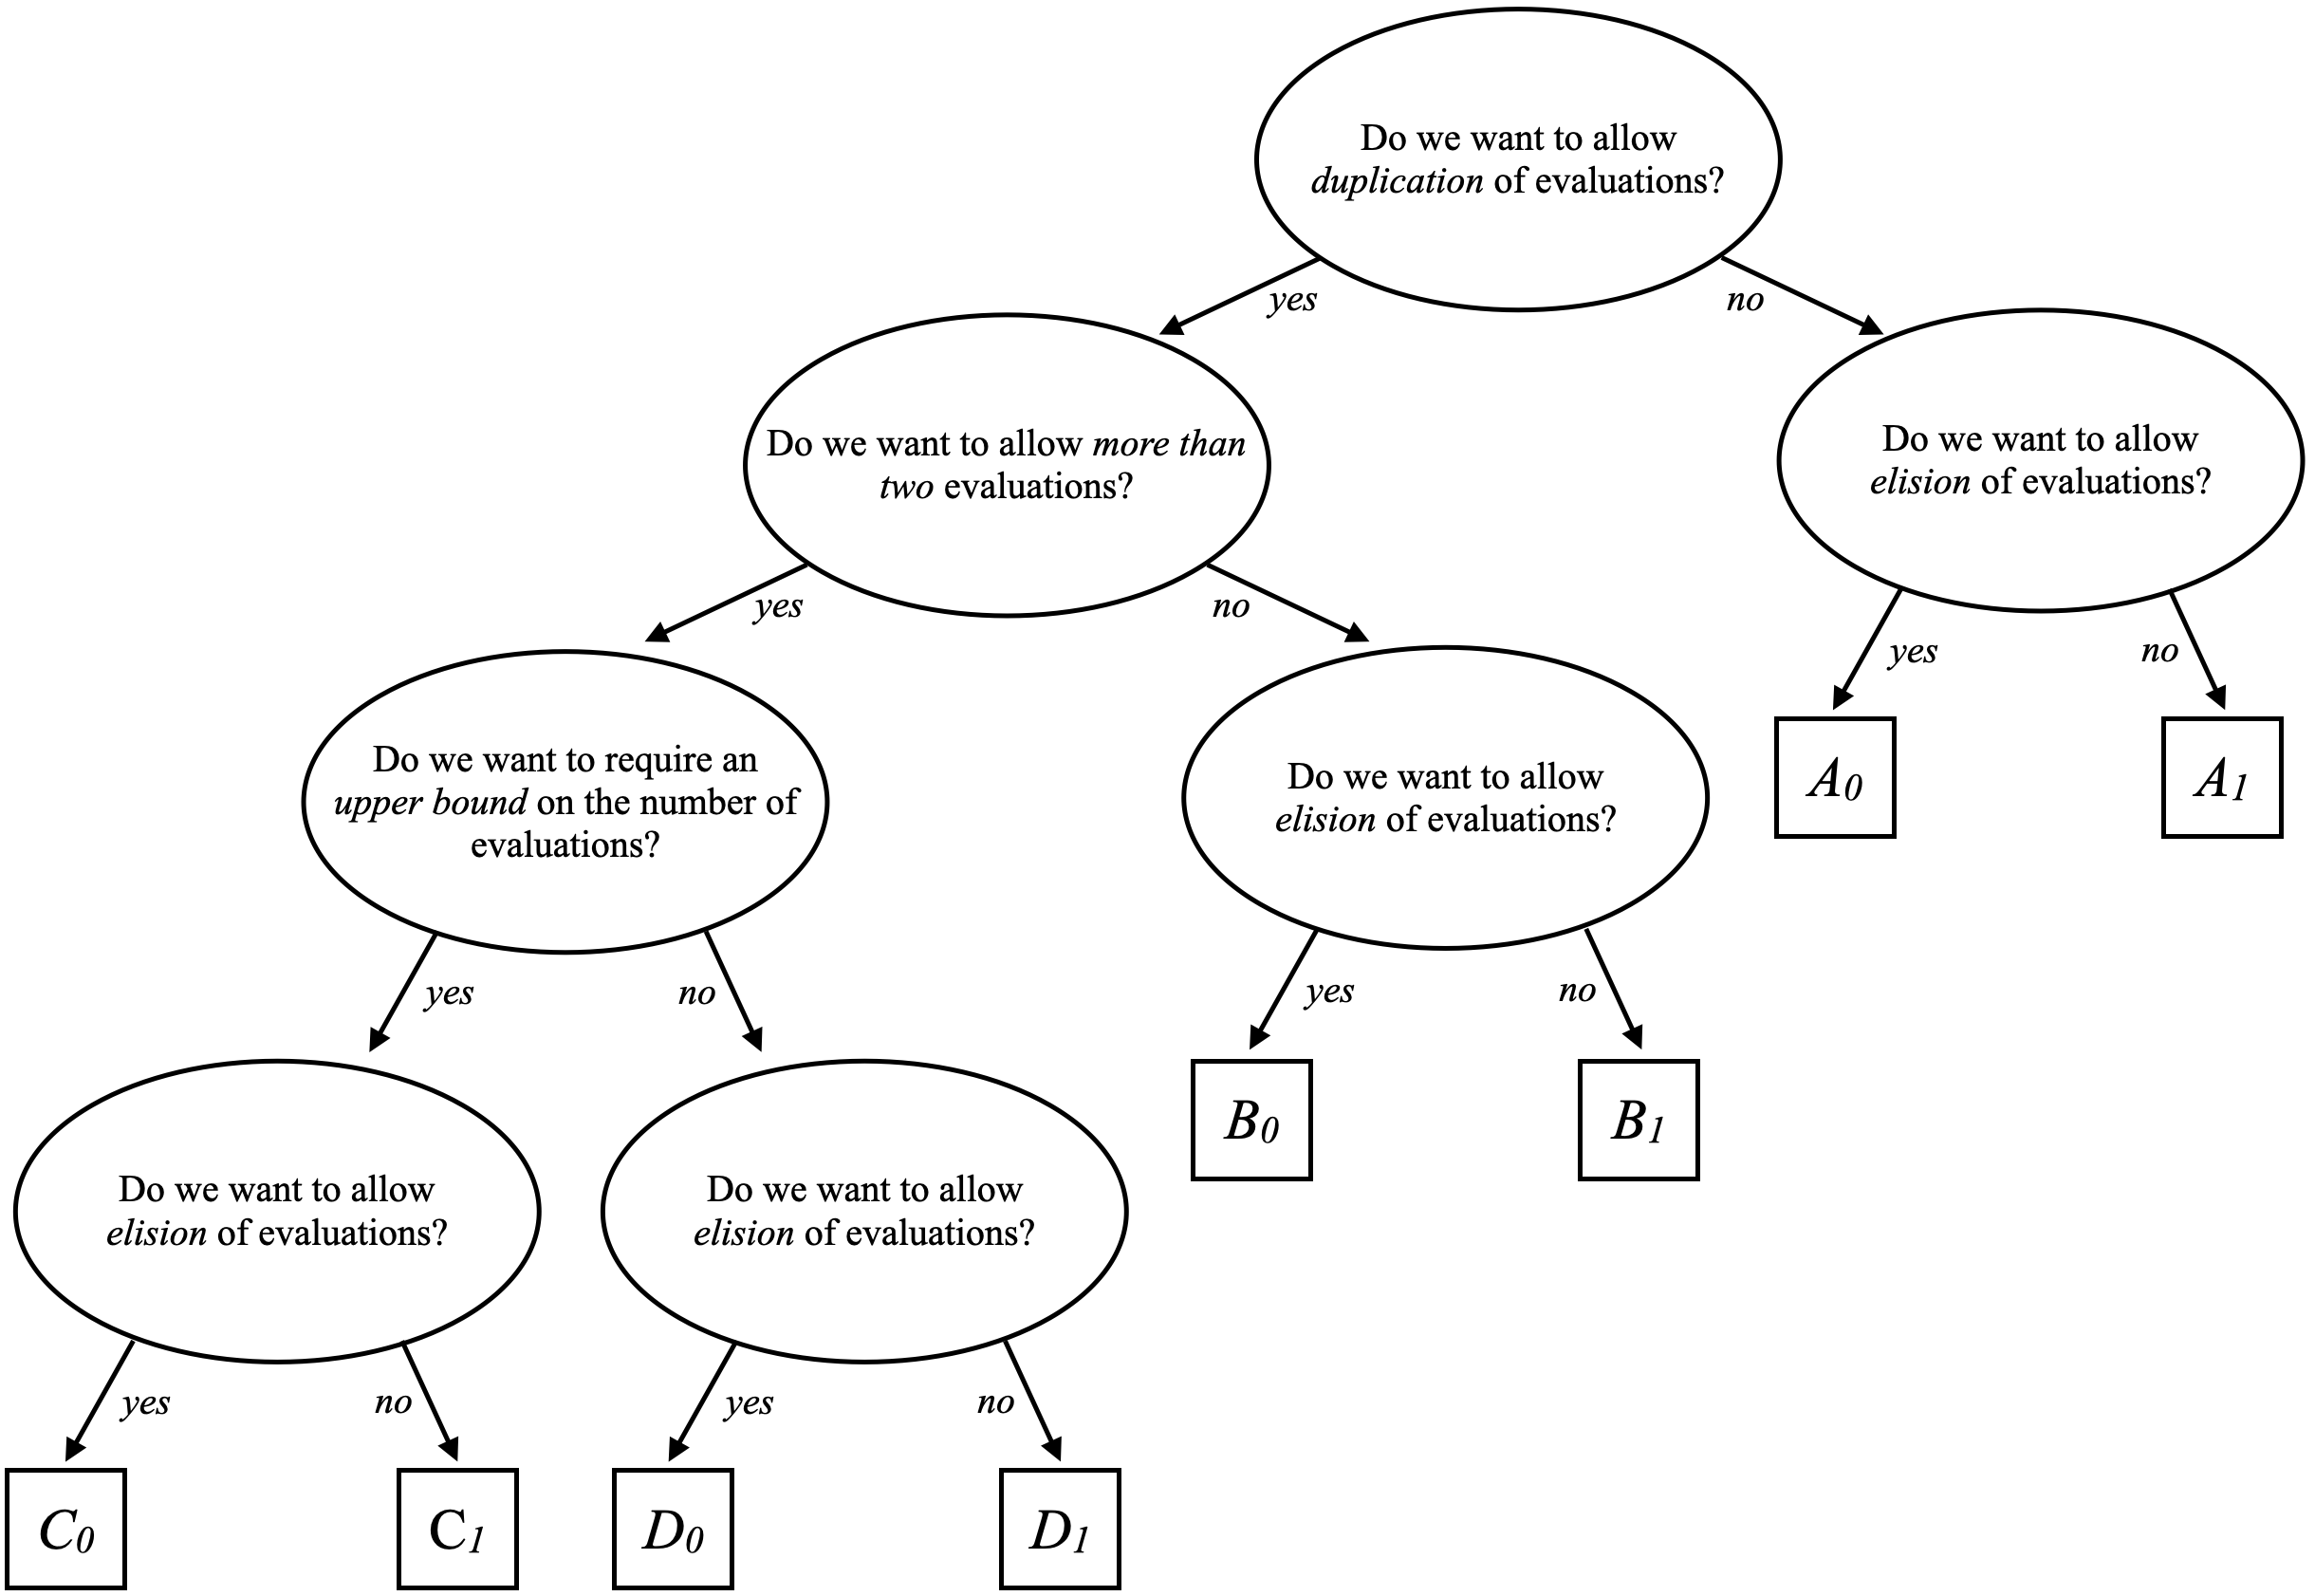
\includegraphics[width=1\linewidth]{images/p3228_fig1.png}
  \vspace{5mm}
  \caption{Possible decision tree for picking a solution.}
  \label{fig:prepost}
\end{figure}

\pagebreak % MANUAL %%%%%%%%%

\renewcommand{\bibname}{References}
\bibliographystyle{abstract}
\bibliography{ref}

%%%%%%%%%%%%%%%%%%%%%%%%%%%%%%%%%%%%%%%%%%%%%

\end{document}
